\section{Introduction}
\begin{frame}{Introduction}
\begin{columns}
\begin{column}{0.5\textwidth}
Motivation
\begin{itemize}
    \item \textit{S. cerevisiae}
    \item Systems biology approach
% Understanding the complexities of life has shown to be challenging. Gene regulation and protein interaction is at the core of shaping the function of any living cell. The interaction networks of proteins and metabolites inside a single cell are complex and ever changing, and it is not always trivial to understand how changes to one or more parts of the network will affect the overall. 
\end{itemize}

The problem
\begin{itemize}
    \item ORFs: 5178 verified, 737 uncharacterized, 689 dubious~\cite{YeastOverview}
    \item TFs: $\sim209$~\cite{Hughes2013}, PKs: $\sim129$~\cite{Rubenstein2007}, PPs: $\sim30$~\cite{Breitkreutz2010}
% Numbers of genes, transcription factors, and protein kinases are still not exactly defined. \textit{S. cerevisiae} currently has 5178 verified open reading frames~(ORFs), 737 uncharacterized ones, and 689 dubious ones~\cite{YeastOverview}.
% Estimated numbers of transcription factors vary from 141 to 251. If we define a transcription factor protein as a protein that binds DNA with sequence-specificity and regulates transcription nearby, then one estimate puts the number of known and putative TFs at 209~\cite{Hughes2013}. Putative refers to proteins that encode DNA-binding domains, and where their regulatory role is not unproven. A count of 127~protein kinases have been studied by Rubenstein~et~al.~\cite{Rubenstein2007}, while 129~protein kinases and 30~phosphatases were characterized by Breitkreutz~et~al.~\cite{Breitkreutz2010}.

    \item Graph learning combining different data types
% to model a cell as a graph to predict how it behaves under different conditions, we first need to infer the graph.
% Studying the abundance of interaction in a cell requires high throughput measurements which still come with the cost of high noise levels. High throughput RNA measurements has become cheaper at an increasing rate and can help in understanding direct protein interactions, as a supplement to directly assaying protein-protein and protein-DNA interaction.
% Since some data types such as RNA measurements are not direct assays of protein-protein and protein-DNA interactions, researchers in the field of systems biology study mathematical models, graph theory, and machine learning to develop ways to take advantage of all the different types of biological data available.
% Inferring graph structure has been examined extensively, each method with different assumptions and limitations. Here, we will try to examine graph structure inference specifically for the case of regulatory networks, and by using data from knockout studies.
\end{itemize}
\end{column}

\begin{column}{0.5\textwidth}
\begin{figure}[ht]
  \centering
  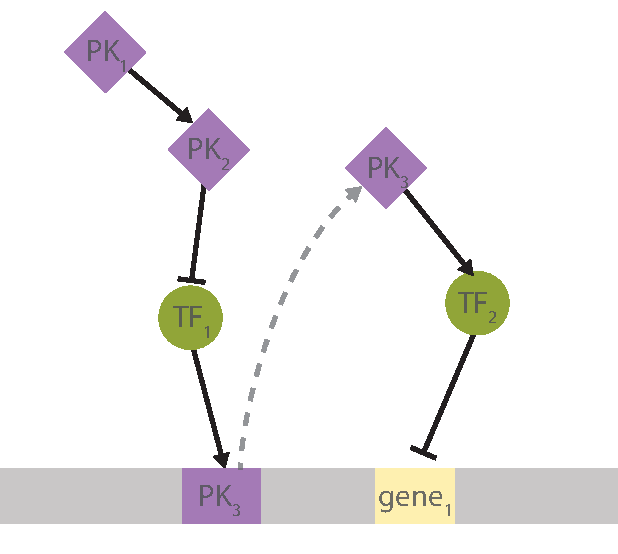
\includegraphics[width=0.7\textwidth]{introduction/fig/problem.pdf}
  \caption{\textbf{Gene regulation.}
  $\pk_1$ regulating $\gene_1$ indirectly through a cascade.}
  \label{fig:problem}
\end{figure}
\end{column}
\end{columns}
\end{frame}


\begin{frame}{Theoretical background}
\begin{columns}
\begin{column}{0.5\textwidth}
% In this section theory and models of gene regulation are discussed, with models used for different types of inference goals and varying assumptions. Relevant previous work leading to the analysis are covered.
Signal transduction
\begin{itemize}
    \item Phosphorylation
% Signal transduction inside the cell is mostly performed through the addition or removal of phosphates as phosphorylation or dephosphorylation of proteins, although there are many other types of signal transduction and protein regulation such as G-protein coupled receptors mediating trans-membrane signals, second messengers such as calcium ions and lipid messengers. 
    \item TF, $\text{KP} = \text{PK} \cup \text{PP}$, V (any genes)
% For intracellular signals leading to gene regulation, gene regulatory proteins can broadly be categorizes as either transcription factors, kinases or phosphatases, where the TFs have direct effects on the gene transcription and kinases and phosphatases regulates the activity of TFs as well as each other. TFs and their regulons, which are the set of genes regulated by a TF, are largely known, while kinase regulation is not as well documented.

% There are about a factor of 10 less phosphatases of yeast than kinases. They have a much smaller specificity in regulation targets and can, to some extent, be seen as serving a general clean-up role by removing phosphates from regulated proteins in order to let cellular signals decay.
% Phosphorylation can generally be seen as a on/off switch for a specific site on the protein, with one state of phosphorylation inducing an active conformation while the other stabilizes a more inactive conformation. It is atypical that a transcription factor will regulate one set of genes while phosphorylated and another while dephosphorylated. It can both be a phosphorylation that activates a proteins function or deactivates it, however since kinases have more specificity, kinase chains will often send a cellular signal when phosphorylated and have the signal decay with dephosphorylation mediated by phosphatases. Proteins are often modeled as either being on or off, but multiple post-translational modifications can have combined effects leading to multiple levels of protein activity for a given protein.
\end{itemize}

Mutant RNA measurements
\begin{itemize}
    \item Gene deletions reveal indirect insight
% indirect insight
    % Gene deletion, or knockouts, can reveal insight into gene regulation even through RNA expression measurements are not a direct assay for protein-DNA or protein-protein interactions.
% figure
    % If the gene expression levels are observed relative to wildtype we can observe how a gene's expression is affected by the presence or absence of a regulator~(\autoref{fig:gene_deletion}). The direct regulation effects of transcription factors are more straightforward than the indirect effects of a protein kinase. Both edges cannot be inferred from any single knockout experiment even for this simple regulation example. By combining the observation in both an experiment with PK deleted and another with the TF deleted the signs of both edges can be determined, where +1 symbolizes activation and -1 repression. In this manner we can infer edges based on gene expression levels observed to be significantly up- or downregulated compared to wildtype in each of these four patters. The example here is simplified to not include any other regulators which can complicate the edge inference, e.g. if there is another regulation pathway that works as a backup for transcription of the regulated gene, so a robust inference method cannot be basing inference on individual regulation paths in isolation.
    
    \item Vital genes
% A protein chosen to be knocked out might be vital to the functioning of the cell, making it impossible to have any mutant cells to observe. When this is the case a researcher can apply a conditional knockout where the gene can be down-regulated in a time-dependent manner so the measurements can be gathered at a specific time after inducing the knockout and before the death of all cells.

% genes where the mutant is not visibly different than wildtype due to low expression of the gene under the tested conditions
% \textbf{Low wildtype expression at tested conditions}

% There can be issues with genes expressed at low levels in the wildtype under the experimental conditions. If the expression is already low for the wildtype it can be difficult to tell the level apart in a knockout mutant given the noise of microarray measurements. For this reason it has been argued~\cite{ChuaPNAS2006} that overexpression of transcription factors is better than knockouts for transcription factors that might not be expressed at the tested environmental conditions. According to their tests overexpression is good enough to produce noticeable changes even for some transcription factors that would normally not be active under the tested environmental conditions.
% A counterpoint can be made with Savageau’s rule of demand~(\autoref{sec:demand_rule}).

    \item Savageau's rule of demand~\cite{Shinar2006}
\label{sec:demand_rule}
% We consider Savageau’s rule of demand which states that high demand genes are generally induced, and low demand genes repressed under typical conditions. Another way of phrasing it is that genes are bound by their regulators at most times. The rule is established empirically as well as from the evolutionary intuition that it creates the highest selection pressure against unfavorable mutations~\cite{Shinar2006}. If it was the opposite case, where genes were generally not bound by their regulators under typical conditions, a mutation of a regulator could have a less noticeable effect. 
\begin{itemize}
    \item KOs are noticeable
% If Savageau's rule of demand holds, a transcription factor will most likely not be expressed at a near undetectable level under typical conditions, so we would expect a knockout of said TF to have a noticeable effect. In the case of overexpression experiments the expression levels will be noticeably different from wildtype if the transcription is not already saturating the target gene promotor. That will typically not be the case for activating TFs where there would be a 2 to 4 fold increase in expression, but in the case of repressors the promotor can be close to saturated and the effect of TF overexpression can be harder to detect.

% If Savageau's rule of demand does \textit{not} hold, so the promotor of a gene is more often bound by a TF under atypical conditions, it will be harder to detect deviation from wildtype expression levels when the TF is under- or overexpressed. TFs responding to stress and alternative carbon sources and their regulons appear to often violate Savageau’s demand rule so their regulation could be missed if not studied under the appropriate conditions.
\end{itemize}
\end{itemize}



\end{column}
\begin{column}{0.5\textwidth}
\begin{figure}[ht]
    \centering
    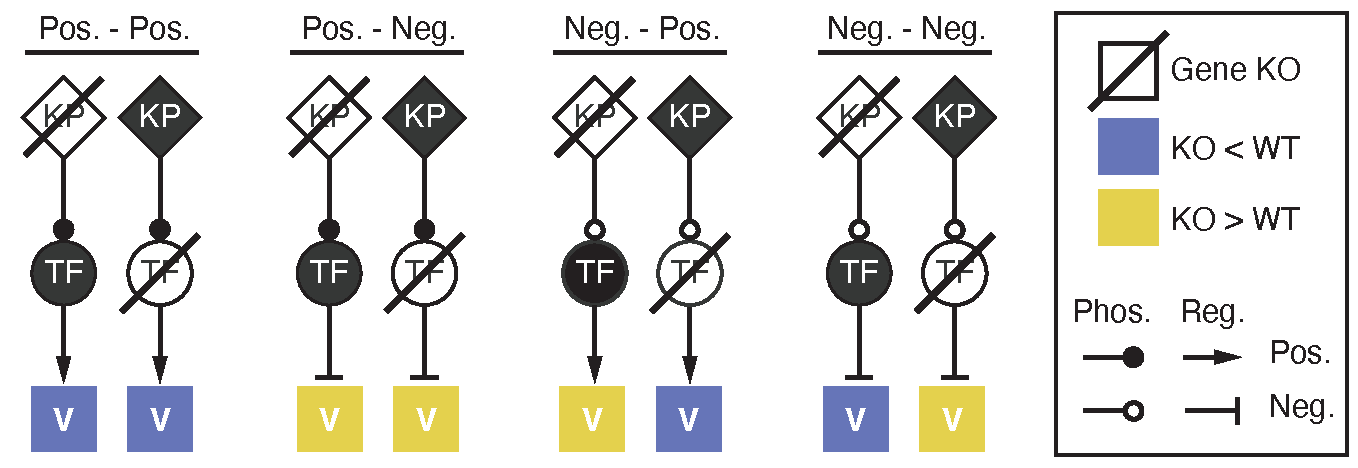
\includegraphics[width=\textwidth]{introduction/fig/Fig1.pdf}
    \caption{\textbf{Effects of gene deletion on gene expression.} Schematic of gene expression levels for a target gene ’V’ relative to wildtype when a gene for either a PK or TF is deleted. All combinations of positive (activating) and negative (repressing) regulation (Pos. or Neg. respectively) are shown. Activating or repressing phosphorylation (Phos.) are indicated with closed or open circles and regulation by TFs (Reg.) are indicated with pointed and flat arrowheads.}
    \label{fig:gene_deletion}
\end{figure}
\end{column}
\end{columns}
\end{frame}




